\documentclass{article}
\usepackage[utf8]{inputenc}
\usepackage{fullpage}
\usepackage[english]{babel}
\usepackage[pdftex]{graphicx}
\usepackage{float}
\usepackage{subcaption}
\usepackage{todonotes}
\usepackage{amsmath}
\usepackage{spverbatim}

\begin{document}

\begin{titlepage}
	\begin{center}
		
\includegraphics[scale=0.4]{epl-logo.jpg} \\[1.5cm]
		\textsc{\LARGE catholic university of louvain-la-neuve} \\[0.5cm]
		\textsc{\Large INGI2143 - Concurrent Systems}\\[2cm]
    		{ \huge \bfseries Report - Assignment 2\\[0.4cm] }
		{\large Alexandre Hauet \\ [0.1cm]Florian Thuin}\\[2cm]
		{\large \today}
	\end{center}
\end{titlepage}

\section{Introduction}

\todo[inline]{Ajouter l'explication de chaque fichier + observations/problèmes }

\section{Minimization of ELECTIONSERVICE vs multiple minimizations}

\begin{tabular}{l|p{0.25\linewidth}|l|l|l}
	Process & Alphabet & Number of states & Minimiz. time & Cum miniz. time \\
    \hline
    ELECTIONSERVICE(3) & [0..2].{close, open} & 740 & 52min & 52min \\
    ABSTRACT0(3) & [0..2].{{close, open}, rcvclaim[0..2], rcvtoken, sndclaim[0..2], sndtoken} & 5652 & 501ms & 501ms \\
    ABSTRACT1(3) & [0..2].{{close, open}, rcvclaim[0..2], {rcvtoken, sndtoken}} & 4826 & 550ms & 1051ms \\
    ABSTRACT2(3) & [0..2].{close, open, rcvtoken, sndtoken} & 2192 & 547ms & 1598ms \\
    ABSTRACT3(3) & [0..2].{close, open, sndtoken} & 1793 & 55ms & 1653ms \\
    ABSTRACT4(3) & [0..2].{close, open} & 740 & 31995ms & 33648ms \\
\end{tabular}

\section{Property OPENCLOSE}
\begin{figure}[h!]
  \centering
    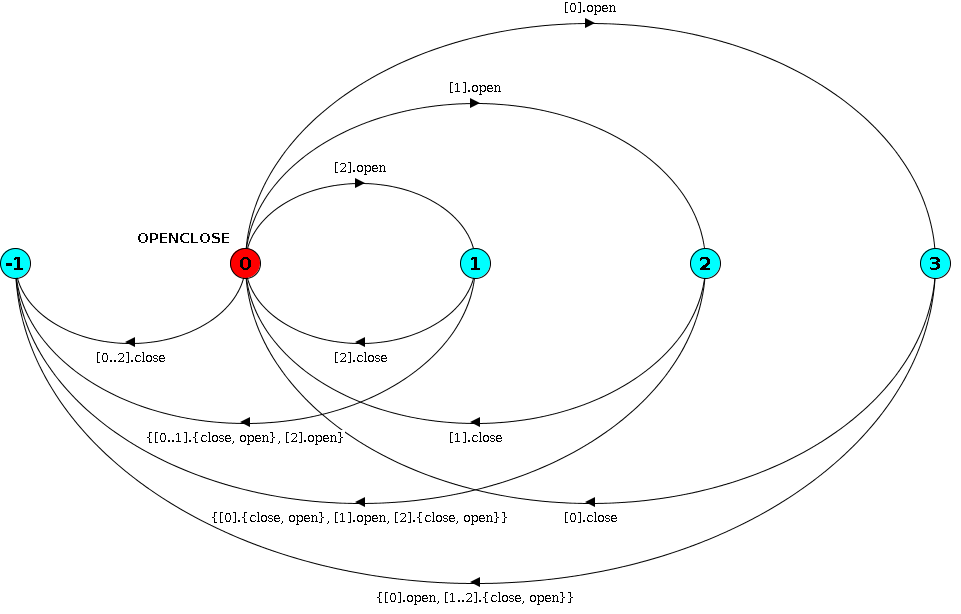
\includegraphics[width=\textwidth]{openclose_lts.png}
    \caption{Picture of the LTS of the property openclose}
\end{figure}

\section{Violation trace for OPENCLOSE on ELECTIONRING(3)}

\begin{figure}[h!]
\begin{equation*}
\begin{split}
	0.sndclaim.0 \rightarrow 1.rcvclaim.0 \rightarrow 0.sndclaim.0 \rightarrow 1.sndclaim.0 \rightarrow 1.rcvclaim.0 \rightarrow \\ 2.rcvclaim.0 \rightarrow 1.sndclaim.0 \rightarrow 2.sndclaim.0 \rightarrow 0.rcvclaim.0 \rightarrow 0.sndtoken \rightarrow \\
    1.rcvtoken \rightarrow \textcolor{red}{1.open} \rightarrow 2.rcvclaim.0 \rightarrow 2.sndclaim.0 \rightarrow 0.rcvclaim.0 \rightarrow \textcolor{red}{0.open}
\end{split}
\end{equation*}
\caption{The violation trace for OPENCLOSE on ELECTIONRING(3)}
\end{figure}

We can see with this trace that two nodes (1 and 0) want to access to the resource at the same time. It's a violation of the propety because the property define that a node can't access to the resource before an other node close it.


\section{CRASHRING LTS}

\todo[inlne]{Afficher le LTS}

\section{ALLFAIR property}

Here is the violation trace for ALLFAIR on ELECTIONRING(3) without fair choice :

\begin{spverbatim}
0.sndclaim.0 -> 1.rcvclaim.0  -> 0.sndclaim.0 -> 1.sndclaim.0 -> 1.rcvclaim.0 -> 0.sndclaim.0 -> 2.rcvclaim.0 -> 1.sndclaim.0 -> 1.rcvclaim.0 -> 2.sndclaim.0 -> 0.rcvclaim.0 -> 0.sndtoken -> 2.rcvclaim.0 -> 1.sndclaim.0 -> 1.rcvtoken -> 0.sndclaim.0 -> 2.sndclaim.0 -> 0.rcvclaim.0 -> 2.rcvclaim.0 -> 1.sndtoken -> 1.rcvclaim.0 -> 0.sndtoken -> 2.sndclaim.0 -> 2.rcvtoken -> 1.sndclaim.0 -> 1.rcvtoken -> 0.sndclaim.0 -> 0.rcvclaim.0 -> 2.sndtoken -> 2.rcvclaim.0 -> 1.sndtoken -> 1.rcvclaim.0 -> 0.sndtoken -> 0.rcvtoken -> 2.sndclaim.0 -> 2.rcvtoken -> 1.sndclaim.0 -> 1.rcvtoken -> 0.sndtoken -> 0.rcvclaim.0 -> 2.sndtoken -> 0.rcvtoken -> 2.rcvclaim.0 -> 1.sndtoken -> 1.rcvtoken -> 0.sndtoken -> 2.sndclaim.0 -> 2.rcvtoken -> 1.sndtoken -> 1.rcvtoken -> 0.sndclaim.0 -> 0.rcvclaim.0 -> 2.sndtoken -> 2.rcvtoken -> 1.sndtoken -> 1.rcvclaim.0 -> 0.sndtoken -> 0.rcvtoken -> 2.sndtoken -> 2.rcvtoken -> 1.sndclaim.0 -> 1.rcvtoken -> 0.sndtoken -> 0.rcvtoken -> 2.sndtoken -> 2.rcvclaim.0 -> 1.sndtoken -> 1.rcvtoken -> 0.sndtoken -> 0.rcvtoken -> 2.sndclaim.0 -> 2.rcvtoken -> 1.sndtoken -> 1.rcvtoken -> 0.sndtoken -> 0.rcvclaim.0 -> 2.sndtoken -> 0.rcvtoken -> 2.sndclaim.2 -> 2.rcvtoken -> 1.sndtoken -> 1.rcvtoken -> 0.sndtoken
\end{spverbatim}
\bigskip

As this trace isn't really readable, the cycle in terminal set is : \newline

\begin{spverbatim}
0.rcvclaim.2 -> 2.sndtoken -> 0.rcvtoken -> 2.sndclaim.2 -> 2.rcvtoken -> 1.sndtoken -> 1.rcvtoken -> 0.sndtoken
\end{spverbatim}
\bigskip

We can explain this result : if the node is always in the election protocol (so never in the \textit{access resources} mode), there isn't any \verb#open# transition. However, it is only possible if there isn't a fair choice between the transition otherwise we would indefintely often access resources and the property ALLFAIR would be respected.

\section{MUTEX violation with increasing number of nodes}

We will not show the N=1 because the property isn't violated. \newline

Without Partial Order Reduction :

\bigskip
\begin{tabular}{l|l|l|l|l}
    N & Number of states & Number of transitions & Time & Length of violation trace \\
    \hline
    2 & 77               & 141                   & 0ms  & 13 \\
    3 & 858              & 2141                  & 1ms  & 17 \\
    4 & 9226             & 29467                 & 17ms & 21 \\
    5 & 117339           & 440519                & 195ms & 25 \\
    6 & 1842823          & 787101009               & 8575ms & 29 \\
\end{tabular}
\bigskip

With Partial Order Reduction :

\bigskip
\begin{tabular}{l|l|l|l|l}
    N & Number of states & Number of transitions & Time & Length of violation trace \\
    \hline
    2 & 74               & 131                   & 8ms   & 13 \\
    3 & 789              & 1753                  & 6ms   & 17 \\
    4 & 8135             & 20496                 & 39ms  & 21 \\
    5 & 96928            & 255807                & 272ms & 25 \\
    6 & 1387005          & 3737714               & 5599ms & 29 \\
\end{tabular}


\section{Checking MUTEX using Supertrace on ELECTIONRING(N)}
\begin{tabular}{l|p{0.25\linewidth}|l|l|l|l}
	N & Number of states & transitions & time & length of violation trace\\
    \hline
    1 & 6   &   7       &   0ms    &   0  \\
    2 & 27  & 49 & 0ms & 49 \\
    3 & 66  & 128 & 0ms & 128 \\
    4 & 123 & 248 & 0ms & 248\\
    5 & 198 & 409 & 1ms & 409\\
    6 & 271 & 597 & 1ms & 496\\
\end{tabular}


\end{document}
